\documentclass[twocolumn]{article}

\usepackage[english]{babel}
\usepackage[a4paper,top=3cm,bottom=3cm,left=3cm,right=3cm,marginparwidth=2.5cm]{geometry}
\usepackage{amssymb}
\usepackage{amsmath}
\usepackage{graphicx}
\usepackage[colorlinks=true, allcolors=blue]{hyperref}
\usepackage{multirow}

\title{Reconsidering repetitions in Ordering Patterns Entropy}
\author{Maximiliano Antonelli, Raúl Eduardo Lopresti, Luciana De Micco and Osvaldo Anibal Rosso}

\begin{document}
\maketitle

\begin{abstract}
Ordering patterns entropy is widely used to detect patterns in time series data. It was successfully applied in medicine, astronomy, economy, human sciences, etc. because is able to detect the causality of data series. Commonly, the arithmetic of the data set is sufficiently fine to suppose that a repetition of a single value in a sub-dataset is improbable, and then repetitions are replaced by ascending values. Also, the presence of noise in data sets forces the introduction of minimum distance to consider that the two samples are different. In this work, we explore the influence of these two factors, coarse grain arithmetics and minimum distance in the ordering patterns entropy and explore the possibility of incorporating those patterns that include repetitions.
\end{abstract}

\section{Introduction}

Let consider a set of symbols $S = \{s_1, s_2, ..., s_N \}$ with a magnitude relation $s_1 < s_2 < ... < s_N$.
Then, a one-dimensional data set of symbols $X = \{x_1, x_2, ..., x_M\}$ with $x_i \in S$ is the data series to explore causality.
In an emmbedding vector $E = \{e_1, e_2, ..., e_{(M-\tau(D-1))}\}$ of dimension $D$ and delay $\tau$, each $e_i$ is a subset of $X$. For instance, if $D = 3$ and $\tau = 2$, $e_1 = \{x_1, x_3, x_5\}, e_2 = \{x_2, x_4, x_6\}, ..., e_{(M-4)} = \{x_{(M-4)}, x_{(M-2)}, x_M\}$.
A set $\Pi = \{\pi_1, \pi_2, ..., \pi_L\}$ is a vector of rankings assigned to each $e_i$. One ranking $\pi_i$ matches univocally with an ordering pattern of $e_i$.

In the Bandt \& Pompe approach \cite{Bandt2002} $N \gg D$, then, the probability of repetition of a symbol from $S$ in an embedding vector $e_i$ is too low and it may be discarded.
In the practice if ${x_i, x_j} \in e_k$ and $x_i = x_j$, the ranking $\pi_i$ is calculated using $x_i > x_j$.

The problem arises when $N \gtrapprox D$, then repetitions appear more frequently and they need to be considered. This set of data commonly appears in voting problems (where symbols are YES, NO, BLANK), binary problems (like WIN, LOSS in games), coarse grain arithmetics and scaling problems in measuring systems, and so on. EXPLICAR MINIMA DISTANCIA PARA VALORES DISTINTOS CUANDO HAY RUIDO

In \ref{Cayley1891}, Cayley introduces their C-trees and the notions of ordering patterns with repetitions. The problem of assigning a rank $\pi_i$ is algorithmically solved in \cite{algorithm306}, this algorithm is more complex than when repetitions are discarded.

%%%%EXPLICAR EL TEMA DE LOS HISTOGRAMAS Y LAS ENTROPÍAS%%%%%%%%%%%%%%%
In this paper, we study the influence of 


\section{Comparing two methods}

In table \ref{tab:comp1} we show all the possible combinations for $S = \{1, 2, 3\}$ and $D=2$ and compare the ranking assigned in each case. We can see that Cayley permutations have more resolution in ordering patterns with repetitions. The embedding vectors are symmetric: three ascending, three descending and three constant, corresponding ordering patterns without repetitions lost this symmetry, but it can be captured by the with-repetitions strategy.


\begin{figure}
    \centering
    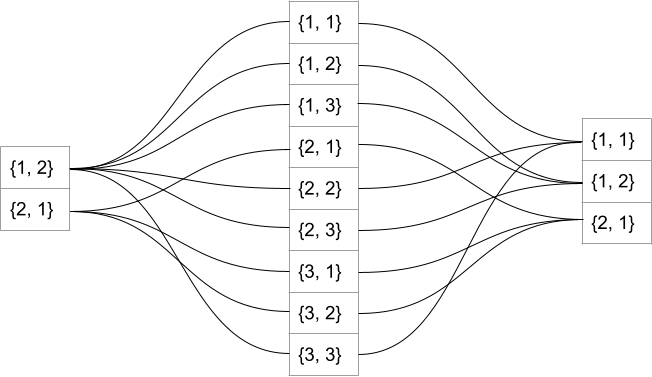
\includegraphics[width=.5\textwidth]{comp_N3_D2.png}
    \caption{Comparison between classical ordering patterns and ordinal patterns with repetitions using $S = \{1, 2, 3\}$ and $D=2$.}
    \label{fig:my_label}
\end{figure}


\begin{table*}[]
\centering
\caption{\label{tab:comp1}Comparison between classical ordering patterns and ordinal patterns with repetitions using $S = \{1, 2, 3\}$ and $D=2$.}
\begin{tabular}{|c|cc|cc|}
\hline
\multirow{2}{*}{\begin{tabular}[c]{@{}c@{}}Emmbedding\\ vector $e_i$\end{tabular}} & \multicolumn{2}{c|}{Without repetitions}                             & \multicolumn{2}{c|}{With repetitions}                                \\ \cline{2-5} 
  & \multicolumn{1}{l|}{Ordering pattern} & \multicolumn{1}{l|}{$\pi_i$} & \multicolumn{1}{l|}{Ordering Pattern} & \multicolumn{1}{l|}{$\pi_i$} \\ \hline
$\{1, 1\}$                                                                         & \multicolumn{1}{c|}{$\{1, 2\}$}       & 1                            & \multicolumn{1}{c|}{$\{1, 1\}$}       & 1                            \\ \hline
$\{1, 2\}$                                                                         & \multicolumn{1}{c|}{$\{1, 2\}$}       & 1                            & \multicolumn{1}{c|}{$\{1, 2\}$}       & 2                            \\ \hline
$\{1, 3\}$                                                                         & \multicolumn{1}{c|}{$\{1, 2\}$}       & 1                            & \multicolumn{1}{c|}{$\{1, 2\}$}       & 2                            \\ \hline
$\{2, 1\}$                                                                         & \multicolumn{1}{c|}{$\{2, 1\}$}       & 2                            & \multicolumn{1}{c|}{$\{2, 1\}$}       & 3                            \\ \hline
$\{2, 2\}$                                                                         & \multicolumn{1}{c|}{$\{1, 2\}$}       & 1                            & \multicolumn{1}{c|}{$\{1, 1\}$}       & 1                            \\ \hline
$\{2, 3\}$                                                                         & \multicolumn{1}{c|}{$\{1, 2\}$}       & 1                            & \multicolumn{1}{c|}{$\{1, 2\}$}       & 2                            \\ \hline
$\{3, 1\}$                                                                         & \multicolumn{1}{c|}{$\{2, 1\}$}       & 2                            & \multicolumn{1}{c|}{$\{2, 1\}$}       & 3                            \\ \hline
$\{3, 2\}$                                                                         & \multicolumn{1}{c|}{$\{2, 1\}$}       & 2                            & \multicolumn{1}{c|}{$\{2, 1\}$}       & 3                            \\ \hline
$\{3, 3\}$                                                                         & \multicolumn{1}{c|}{$\{1, 2\}$}       & 1                            & \multicolumn{1}{c|}{$\{1, 1\}$}       & 1                            \\ \hline
\end{tabular}
\end{table*}


In table \ref{tab:comp2} we use $S = \{1, 2\}$ and $D=2$. The permitted ordering patterns are $L_1 = 2$ when repetitions are discarded and $L_2 = 3$ when repetitions are taken into account.

\begin{figure}
    \centering
    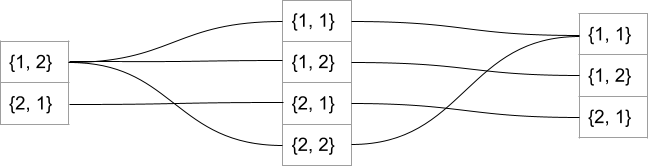
\includegraphics[width=.5\textwidth]{comp_N2_D2.png}
    \caption{Comparison between classical ordering patterns and ordinal patterns with repetitions using $S = \{1, 2\}$ and $D=2$.}}
    \label{fig:my_label}
\end{figure}

\begin{table*}[]
\centering
\caption{\label{tab:comp2}Comparison between classical ordering patterns and ordinal patterns with repetitions using $S = \{1, 2\}$ and $D=2$.}
\begin{tabular}{|c|cc|cc|}
\hline
\multirow{2}{*}{\begin{tabular}[c]{@{}c@{}}Emmbedding\\ vector $e_i$\end{tabular}} & \multicolumn{2}{c|}{Without repetitions}                             & \multicolumn{2}{c|}{With repetitions}                                \\ \cline{2-5} 
                                                                                   & \multicolumn{1}{l|}{Ordering pattern} & \multicolumn{1}{l|}{$\pi_i$} & \multicolumn{1}{l|}{Ordering Pattern} & \multicolumn{1}{l|}{$\pi_i$} \\ \hline
$\{1, 1\}$                                                                         & \multicolumn{1}{c|}{$\{1, 2\}$}       & 1                            & \multicolumn{1}{c|}{$\{1, 1\}$}       & 1                            \\ \hline
$\{1, 2\}$                                                                         & \multicolumn{1}{c|}{$\{1, 2\}$}       & 1                            & \multicolumn{1}{c|}{$\{1, 2\}$}       & 2                            \\ \hline
$\{2, 1\}$                                                                         & \multicolumn{1}{c|}{$\{2, 1\}$}       & 2                            & \multicolumn{1}{c|}{$\{2, 1\}$}       & 3                            \\ \hline
$\{2, 2\}$                                                                         & \multicolumn{1}{c|}{$\{1, 2\}$}       & 1                            & \multicolumn{1}{c|}{$\{1, 1\}$}       & 1                            \\ \hline
\end{tabular}
\end{table*}

In table \ref{tab:comp3} we use $S = \{1, 2\}$ and $D=3$. The permitted ordering patterns are $L_1 = 6$ when repetitions are discarded and $L_2 = 27$ when repetitions are taken into account. This table shows a new consideration to consider when $N < D$, only a few patterns $\pi_i$ can represent an embedding vector $e_i$ from the data set $X$.

\begin{figure}
    \centering
    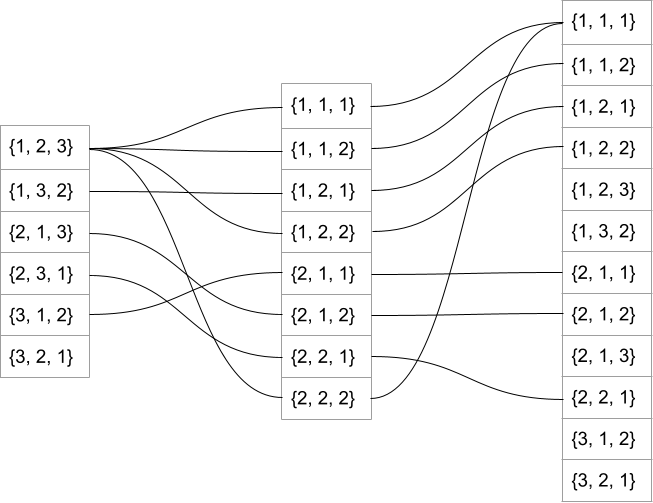
\includegraphics[width=.5\textwidth]{comp_N2_D3.png}
    \caption{Comparison between classical ordering patterns and ordinal patterns with repetitions using $S = \{1, 2\}$ and $D=3$}
    \label{fig:my_label}
\end{figure}

\begin{table*}[]
\centering
\caption{\label{tab:comp3}Comparison between classical ordering patterns and ordinal patterns with repetitions using $S = \{1, 2\}$ and $D=3$.}
\begin{tabular}{|c|cc|cc|}
\hline
\multirow{2}{*}{\begin{tabular}[c]{@{}c@{}}Emmbedding\\ vector $e_i$\end{tabular}} & \multicolumn{2}{c|}{Without repetitions}                             & \multicolumn{2}{c|}{With repetitions}                                \\ \cline{2-5} 
                                                                                   & \multicolumn{1}{l|}{Ordering pattern} & \multicolumn{1}{l|}{$\pi_i$} & \multicolumn{1}{l|}{Ordering Pattern} & \multicolumn{1}{l|}{$\pi_i$} \\ \hline
$\{1, 1, 1\}$                                                                      & \multicolumn{1}{c|}{$\{1, 2, 3\}$}    & 1                            & \multicolumn{1}{c|}{$\{1, 1, 1\}$}    & 1                            \\ \hline
$\{1, 1, 2\}$                                                                      & \multicolumn{1}{c|}{$\{1, 2, 3\}$}    & 1                            & \multicolumn{1}{c|}{$\{1, 1, 2\}$}    & 2                            \\ \hline
$\{1, 2, 1\}$                                                                      & \multicolumn{1}{c|}{$\{1, 3, 2\}$}    & 2                            & \multicolumn{1}{c|}{$\{1, 2, 1\}$}    & 4                            \\ \hline
$\{1, 2, 2\}$                                                                      & \multicolumn{1}{c|}{$\{1, 2, 3\}$}    & 1                            & \multicolumn{1}{c|}{$\{1, 2, 2\}$}    & 5                            \\ \hline
$\{2, 1, 1\}$                                                                      & \multicolumn{1}{c|}{$\{3, 1, 2\}$}    & 5                            & \multicolumn{1}{c|}{$\{2, 1, 1\}$}    & 10                           \\ \hline
$\{2, 1, 2\}$                                                                      & \multicolumn{1}{c|}{$\{2, 1, 3\}$}    & 4                            & \multicolumn{1}{c|}{$\{2, 1, 2\}$}    & 11                           \\ \hline
$\{2, 2, 1\}$                                                                      & \multicolumn{1}{c|}{$\{2, 3, 1\}$}    & 3                            & \multicolumn{1}{c|}{$\{2, 2, 1\}$}    & 13                           \\ \hline
$\{2, 2, 2\}$                                                                      & \multicolumn{1}{c|}{$\{1, 2, 3\}$}    & 1                            & \multicolumn{1}{c|}{$\{1, 1, 1\}$}    & 1                           \\ \hline
\end{tabular}
\end{table*}

\begin{figure}[h]
  \centering
  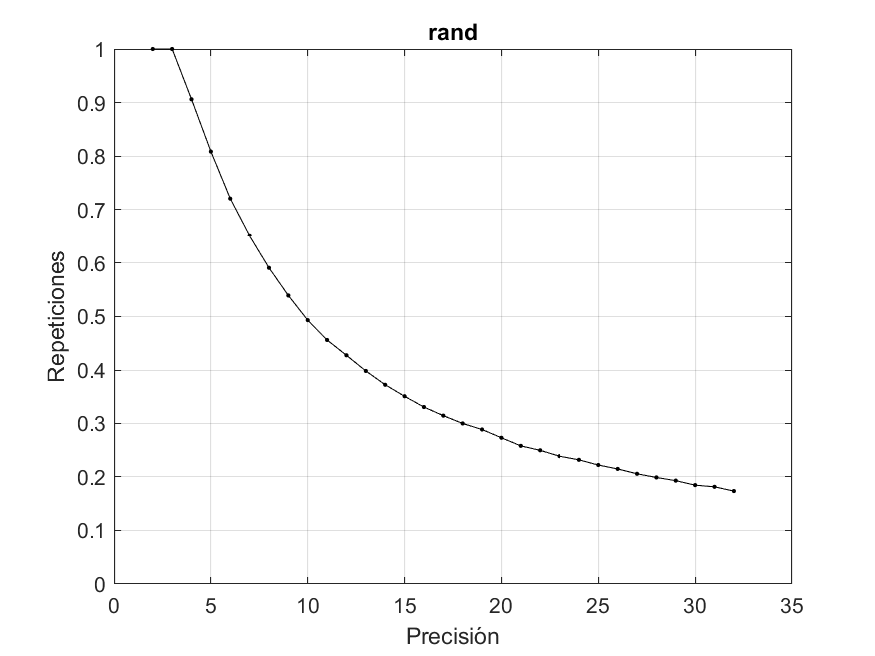
\includegraphics[width=.5\textwidth]{randReps.png}
  \caption{Probabilidad de encontrar un símbolo repetido en una palabra de emmbedding para $D = 4$}
  \label{fig:randReps}
\end{figure}
\begin{figure}[h]
  \centering
  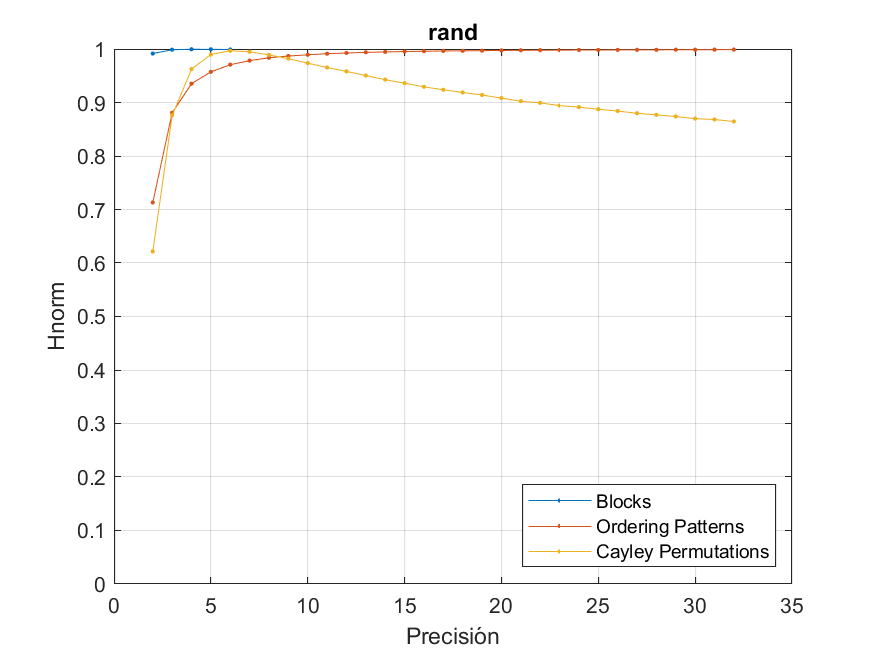
\includegraphics[width=.5\textwidth]{randCuantis.png}
  \caption{Valor de los tres cuantificadores en función de la precisión para D = 4}
  \label{fig:randCuantis}
\end{figure}
\begin{figure}[h]
  \centering
  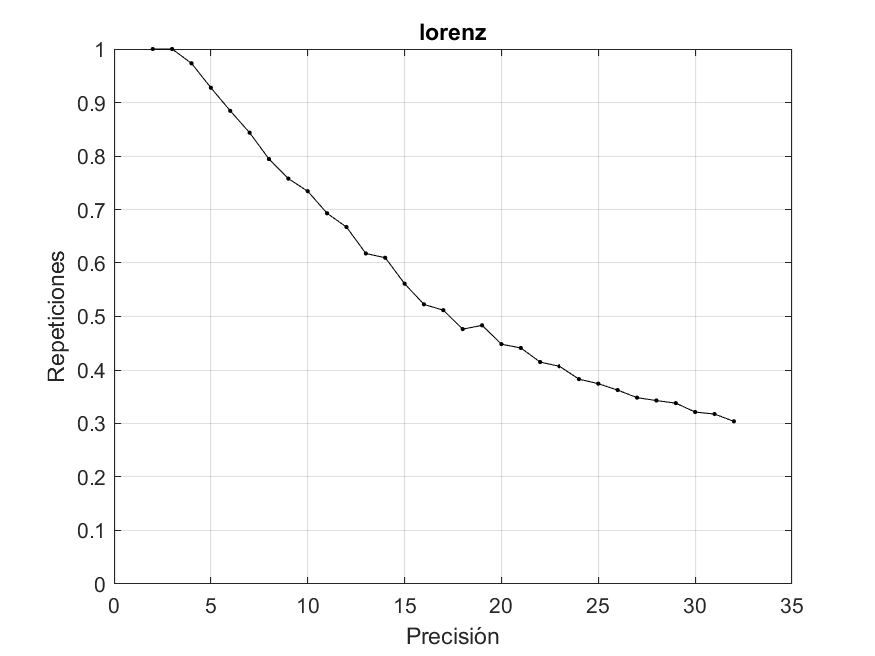
\includegraphics[width=.5\textwidth]{lorenzReps.png}
  \caption{Probabilidad de encontrar un símbolo repetido en una palabra de emmbedding para $D = 4$}
  \label{fig:lorenzReps}
\end{figure}
\begin{figure}[h]
  \centering
  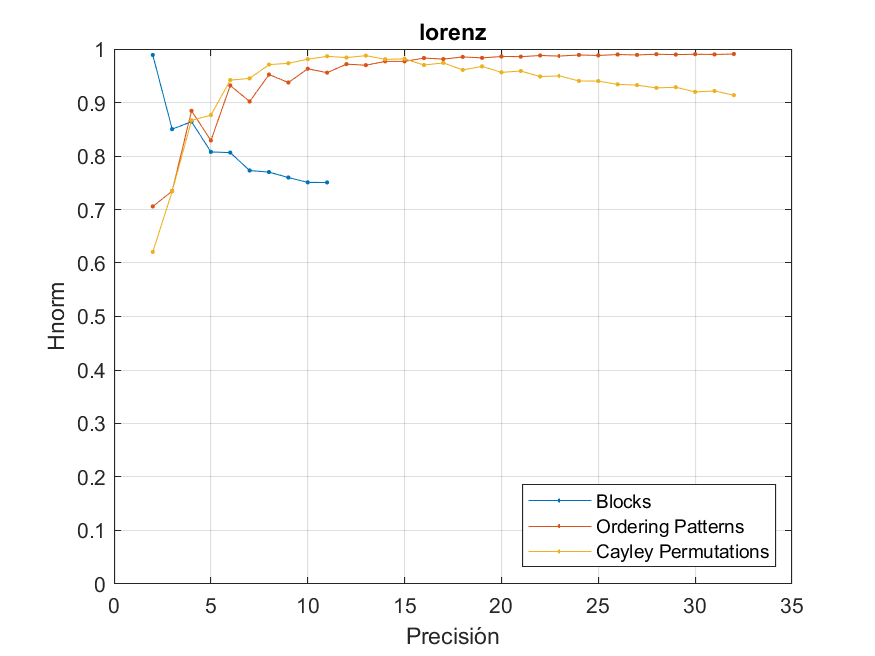
\includegraphics[width=.5\textwidth]{lorenzCuantis.png}
  \caption{Valor de los tres cuantificadores en función de la precisión para D = 4}
  \label{fig:randCuantis}
%%% EXPLICAR EL TEMA DE LOS PATRONES DE ORDEN NO ALCANZABLES, LOS HISTOGRAMAS Y LAS ENTROPÍAS%%%%%%%%%%%%%%

%%% TAMBIÉN SURGE EL SIGUIENTE PROBLEMA, UNA SERIE CON MÁXIMA ENTROPÍA DE PATRONES VERÁ REDUCIDA SU ENTROPÍA PARA UNA PRESICIÓN NUMÉRICA DADA, PERO OTRA SERIE EN DONDE ALGÚN PATRÓN ES MENOS PROBABLE PUEDE TENER MAYOR ENTROPÍA PARA ESA MISMA PRECISIÓN. ESTO SE DEBE A LA ASIMETRÍA CON LA QUE SON ASIGNADOS LOS RANKINGS CUANDO LA AMPLITUD SE DESCARTA Y TAMBIÉN A LA FALTA DE UN SÍMBOLO PARA LOS PATRONES CON REPETICIÓN.%%%

\end{figure}
\section{Consequences on Entropy and Disequilibrium}

\begin{figure}
    \centering
    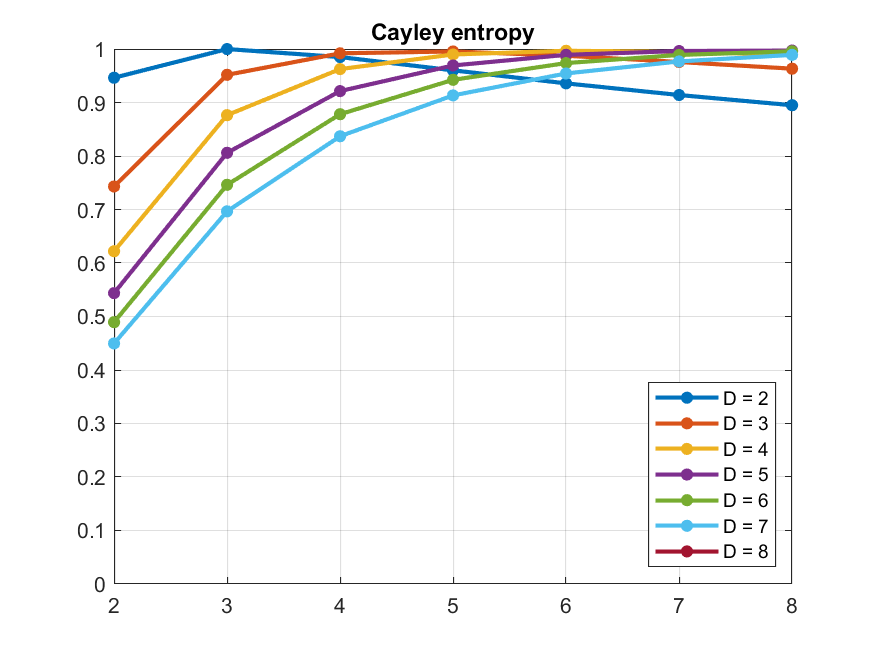
\includegraphics[width=.5\textwidth]{cayleyHvsN.png}
    \caption{Caption}
    \label{fig:cayleyvsN}
\end{figure}

\begin{figure}
    \centering
    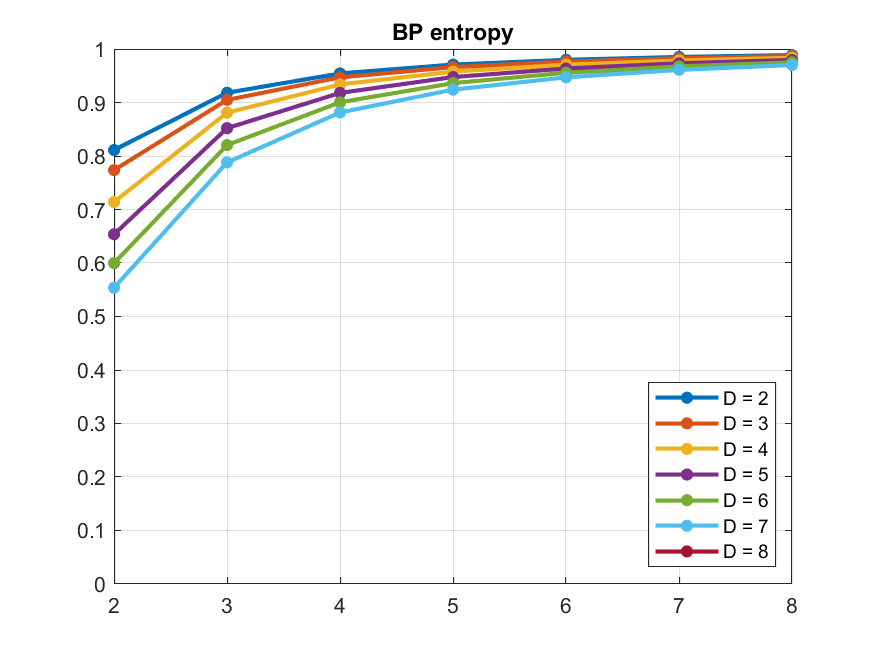
\includegraphics[width=.5\textwidth]{bpHvsN.png}
    \caption{Caption}
    \label{fig:bpvsN}
\end{figure}

\section{Discarding unreachable patterns}

\begin{figure}
    \centering
    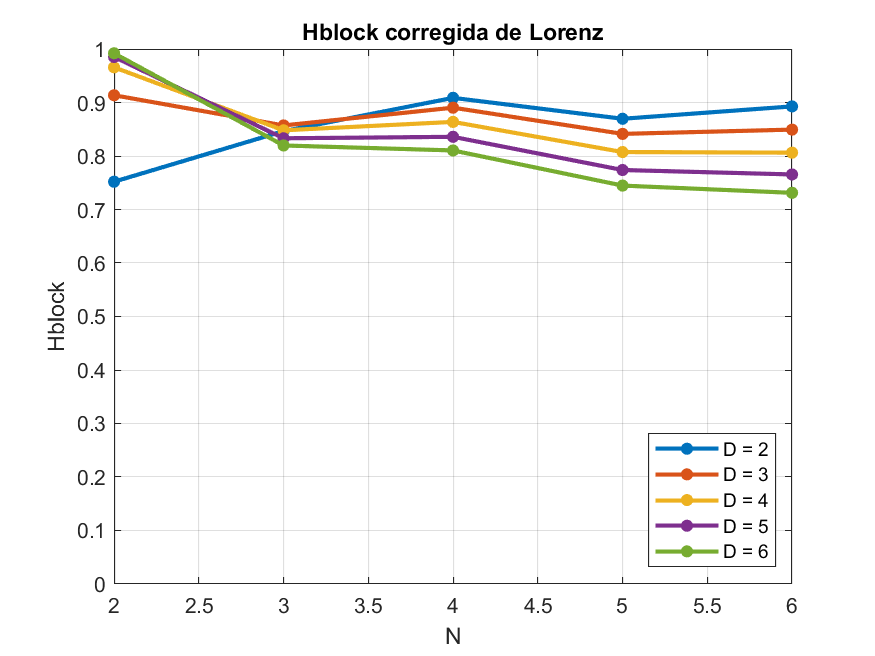
\includegraphics[width=.5\textwidth]{blockHlorenzCorreg.png}
    \caption{Enter Caption}
    \label{fig:enter-label}
\end{figure}

\begin{figure}
    \centering
    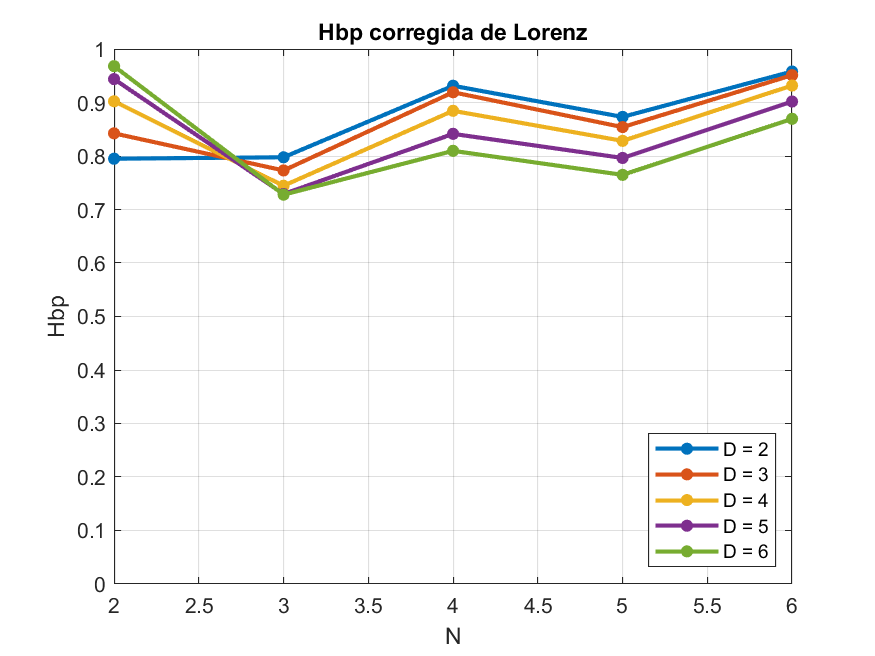
\includegraphics[width=.5\textwidth]{bpHlorenzCorreg.png}
    \caption{Enter Caption}
    \label{fig:enter-label}
\end{figure}

\begin{figure}
    \centering
    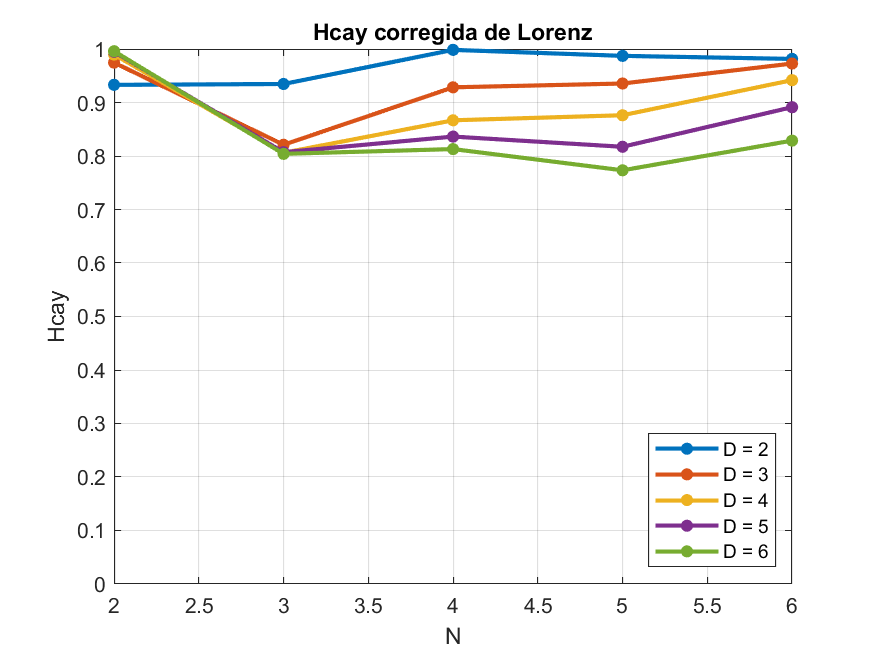
\includegraphics[width=.5\textwidth]{cayHlorenzCorreg.png}
    \caption{Enter Caption}
    \label{fig:enter-label}
\end{figure}


\bibliographystyle{alpha}
\bibliography{sample}

\end{document}